\section{Introduction}

When modeling high-dimensional high-dimensional where the number of features \(p\) exceeds
the number of observations \(n\), it is impossible to apply classical statistical models
such as standard linear regression since the design matrix \(\mat X\) is no longer of full
rank. A common remedy to this problem is to \emph{regularize} the model by adding a term to
the objective function that punishes models with large coefficients (\(\vec\beta\)). If we
let \(g(\vec\beta; \mat X, \vec y)\) be the original objective function---which when
minimized improves the model's fit to the data (\(\mat X, \vec y\))---then we are
interested in minimizing the following objective:
\begin{equation}
  \label{eq:general-objective}
  f(\beta_0, \vec\beta; \mat X, \vec y) = g(\beta_0, \vec\beta; \mat X, \vec y) + h(\vec\beta),
\end{equation}
which is composed of \(g\) and a penalty term \(h(\vec\beta)\) that depends only on \(\bm{\beta}\).
Some of the most common penalties are the \(\ell_1\) norm (\(\lVert \vec\beta \rVert_1\)) and squared \(\ell_2\) norm
penalties (\(\lVert \bm{\beta} \rVert_2^2\)), which if \(g\) is the standard ordinary least-squares objective, represent
the lasso~\citep{tibshirani1996,santosa1986,donoho1994} and ridge (Tikhonov) regression
% TODO: insert reference for ridge regression
respectively. Other common penalties include the sorted \(\ell_1\)-norm used in Sorted
L-One Penalized Estimation (SLOPE)~\citep{bogdan2013,zeng2014,bogdan2015}, the
minimax-concave penalty (MCP)~\citep{zhang2010}, hinge loss (used in support vector
machines~\citep{cortes1995}) and smoothly-clipped absolute
deviation~(SCAD)~\citep{fan2001}. Many penalities---indeed all of the mentioned
ones---shrink coefficients in proportion to their sizes.

The issue with this type of shrinkage is that it is sensitive to the scales of the features
in \(\mat X\). To avoid this it is common to \emph{normalize} the features before fitting
the model by shifting and scaling each feature by measures of location and scale
respectively. For some problems such measures arise naturally from contextual knowledge
about the problem, but in most cases they must be estimated from data. A popular strategy
is to use the mean and standard deviation of each feature as location and scale factors
respectively, which is called \emph{standardization}. Most types of normalization are based
only on the marginal distributions of the features, but there are exceptions such as the
adaptive lasso~\citep{zou2006}. Another reason for normalizing the features is to improve
properties of optimization algorithms used to fit the model, but we will not consider this
topic here.

The choice of normalization may have consequences for the estimated model. As a first
example of this, consider \Cref{fig:realdata-paths}, which displays the lasso paths for
four real data sets and two different types of normalization. For most of the datasets, the
models differ significantly depending on type of normalization, yielding differences in
terms of feature selection as well as signs and magnitudes of the corresponding
coefficients.

\begin{figure}[bpt]
  \centering
  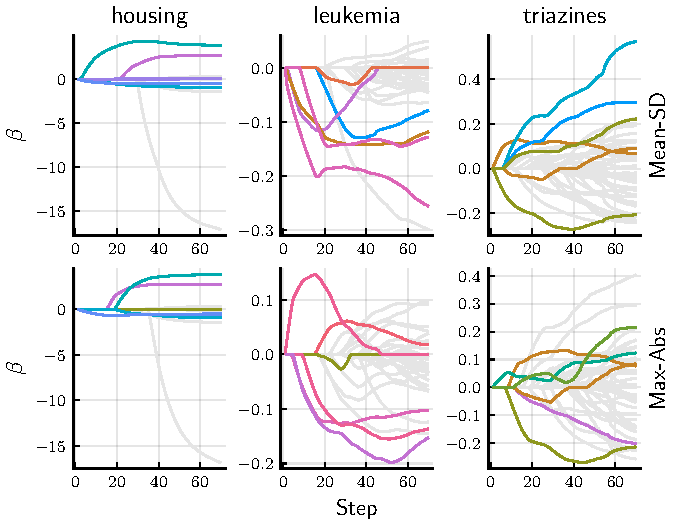
\includegraphics[]{plots/realdata_paths.pdf}
  \caption{%
    Lasso paths for real datasets using two types of normalization:
    standardization and maximum absolute value normalization (max--abs). We have fit
    the lasso path to four different datasets:
    \data{housing}~\citep{harrison1978}, \data{leukemia}~\citep{golub1999},
    \data{triazines}~\citep{king}, and \data{w1a}~\citep{platt1998}. (See \Cref{sec:data-summary}
    for more information about these data sets.) For each
    dataset, we have colored the coefficients if they were among the first five
    to become non-zero under either of the two normalization schemes. We see
    that the paths differ with regards to the size as well as the signs of the
    coefficients, and that, in addition, the features to become active first
    differ between the normalization types.
  }
  \label{fig:realdata-paths}
\end{figure}

In spite of this relationship between normalization and regularization, there has so far
been no research on the topic. Instead, the choice of normalization is often motivated by
being standard. And sometimes the choice is based on computational aspects such as
optimization performance and data storage. At the time of writing, for instance, the
popular machine learning library \texttt{scikit-learn}~\citep{scikit-learndevelopers2024}
recommends maximum absolute value normalization in the particular case of sparse data. Yet,
as we have already seen (\Cref{fig:realdata-paths}), this may have dramatic effects for the
results.

Standardization is a natural choice when the features are normally distributed. But for
other types of data the choice is not as straightforward. There is for instance no clear
approach to normalizing binary features (where the each observations takes either of only
two values). Anecdotal suggestions include not normalizing at all or to normalize as you
would if it were continuous data---the implications of either of these suggestions (or in
deed any other), however, have yet to be investigated.

In this paper we will begin to bridge this knowledge gap by studying normalization in the
context of binary data. We will focus on three models that each correspond to a particular
case of \Cref{eq:general-objective}: the lasso, ridge, and elastic net~\citep{zou2005}. The
latter of these, the elastic net, is a generalization of the previous two, and is
represented by the following optimization problem
%
\begin{equation}
  \label{eq:elastic-net}
  \operatorname*{minimize}_{\beta_0 \in \mathbb{R},\vec{\beta} \in \mathbb{R}^p}\left( f(\beta_0, \vec{\beta};\vec{X},\vec{y},\lambda_1,\lambda_2)=\frac{1}{2} \lVert \vec y - \beta_0 - \tilde{\mat{X}}\vec{\beta} \rVert^2_2  + \lambda_1 \lVert \vec\beta \rVert_1 + \frac{\lambda_2}{2}\lVert \vec \beta \rVert_2^2\right).
\end{equation}
%
Setting \(\lambda_1 = 0\) results in the ridge regression objective, whereas \(\lambda_2 =
0\) gives us the lasso. These methods are staples in the field of statistics and machine
learning and are accompanied by a large body of theoretical work and applications for real
data.

We pay particular attention to the case when binary features are imbalanced, that is, have
relatively many ones or zeroes. In this scenario, we demonstrate that the choice of
normalization directly influences the estimated regression coefficients and that this
effect is different for the lasso and ridge regression. In the case of the lasso, we show
that this bias can be mitigated by scaling with variance but that this comes at the cost of
increased variance. For ridge regression we show that scaling by standard deviation
achieves the same effect. In the case of the elastic net, however, we show that there is no
simple normalization method that can mitigate this bias but that it is possible to
circumvent it by instead weighting the penalty terms in the elastic net.

We also study the case of mixed data and show that the choice of normalization has implicit
consequences for the relative weighting of binary and normal features, even in the case
when the binary features are balanced. If we believe, for instance, that a unit change in
the binary variable should equal a certain change in the normal variable (say, two standard
deviations), then scaling must be modified to take this into account.

% TODO: complete this paragraph
Finally, we look at a simple case of interactions between normal and binary features, and
demonstrate what?

